\documentclass[10pt,dvipdfmx]{standalone}
% \documentclass[dvipdfmx,b5paper,papersize]{jsarticle}
\usepackage{tikz}
\usetikzlibrary{intersections, calc}
\usetikzlibrary{arrows.meta}
\usepackage{physics}


\begin{document}

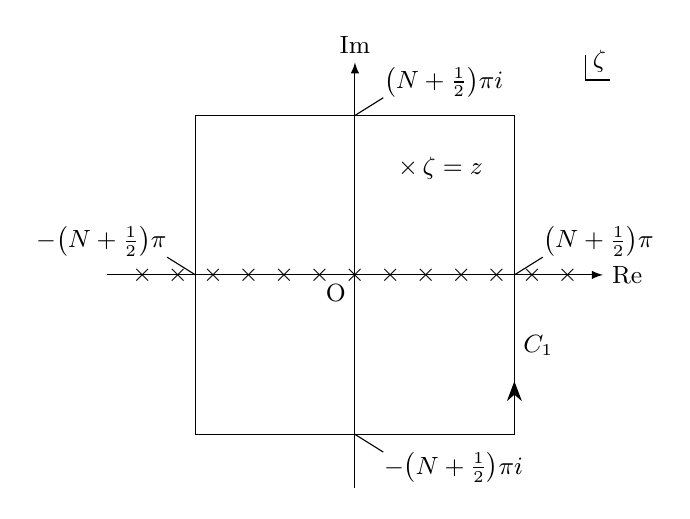
\begin{tikzpicture}[x=4.5mm,y=4.5mm,>=latex]
  \small % 文字サイズ
  % \scriptsize

  % 座標系
  \draw[->] (-7,0) -- (7, 0) node[right]{$\Re$}; % x軸
  \draw[->] (0,-6) -- (0, 6) node[above]{$\Im$}; % y軸
  \node(O) at (0,0) [below left]{O}; % 原点
  % 右上
  \def\ztx{6.5}
  \def\zty{5.5}
  \def\ztd{0.7}
  \draw (\ztx+\ztd,\zty) -- (\ztx,\zty) -- (\ztx,\zty+\ztd);
  \node at (\ztx,\zty) [above right=-0.5pt] {$\zeta$};

  % 特異点
  \def\batsu{{\small $\times$}}
  % x軸上
  \foreach \x in {-6,...,6} {
    \node(O) at (\x,0) {\batsu};
  }
  % zeta = z
  \path (1.5,3) coordinate (z) node{\batsu} node[right=2pt]{$\zeta=z$};

  % 四角
  \def\a{4.5}
  \draw[] (-\a,-\a) -- (-\a,\a) -- (\a,\a) -- (\a,-\a) -- (-\a,-\a);
  % 矢印
  \draw[arrows= {-Stealth[scale=1.5]}] (\a,-\a) -- (\a, -3);
  % C
  \node at (\a,-2) [right]{$C_1$};

  % 座標
  \def\dx{0.8}
  \def\dy{0.5}
  \draw (\a,0) -- (\a+\dx,\dy) node[above right=-3pt] {$\qty(N+\frac12)\pi $}; % 右
  \draw (-\a,0) -- (-\a-\dx,\dy) node[above left=-3pt] {$-\qty(N+\frac12)\pi $}; % 左
  \draw (0,\a) -- (\dx,\a+\dy) node[above right=-3pt] {$\qty(N+\frac12)\pi i$}; % 上
  \draw (0,-\a) --(\dx,-\a-\dy) node[below right=-3pt] {$-\qty(N+\frac12)\pi i$}; % 下

  % テンプレ
  % \fill (2,1) coordinate (P) circle[radius=2pt] node[right=2pt] {P};

\end{tikzpicture}



\if0
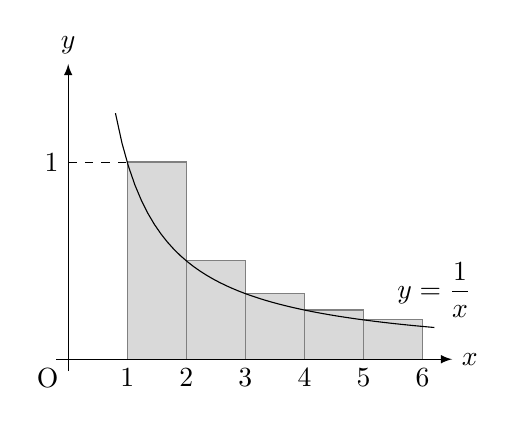
\begin{tikzpicture}[x=0.75cm,y=2.5cm,>=latex]
  \def\width{1.0};
  \def\s{1.5};
  \def\n{6};
  \def\domain{0.8:\n*\width+0.2};
  \def\fx{1/\x};

  \node(O) at (0,0) [below left]{O}; % 原点
  \path [name path=graph, domain=\domain, samples=50] plot(\x, \fx);
  \foreach \x in {0,...,4} {
    \path[name path global/.expanded=path-\x](\width+\width*\x,0) -- (\width+\width*\x,1.1); % 縦棒。関数によって範囲を調整。足りないとエラー、長すぎると図の上に空白が。
    \path[name intersections={of=graph and path-\x}]; % 交点求める
    \coordinate (p-\x) at (intersection-1); % 交点
    \filldraw[fill=gray!30,draw=gray] ($(0,0)!(p-\x)!(1,0)$) rectangle ($(p-\x)+(\width,0)$); %長方形を描く
  }
  \foreach \x in {1,...,\n} { % x軸目盛り
    \node(O) at (\x*\width,0) [below]{$\x$};
  }
  \node(O) at (0,1) [left]{$1$}; % y軸目盛り
  \draw[->] (-0.2,0) -- (\n*\width+0.5, 0) node[right]{$x$};
  \draw[->] (0,-0.2*0.75/2.5) -- (0, 1.5) node[above]{$y$};
  \draw [domain=\domain, samples=50] plot(\x, \fx) node[above]{$\displaystyle y=\frac1x$}; % 短冊の上に draw したいので、短冊drawコマンドの後に書く
  \draw [dashed] (0,1) -- (1,1);
\end{tikzpicture}

\fi


\end{document}